% Chapter 3

\chapter{Hybrid Methods} % Main chapter title

\label{Chapter3} % For referencing the chapter elsewhere, use \ref{Chapter2} 
%%%%%%%%%%%%%%%%%%%%%%%%%%%%%%%%%%%%%%%%%%%%%%%%%%%%%%%%%%%%%%%%%%%%%%%%%%%%%%%
% Hybrid classical-quantum annealing algorithm
%%%%%%%%%%%%%%%%%%%%%%%%%%%%%%%%%%%%%%%%%%%%%%%%%%%%%%%%%%%%%%%%%%%%%%%%%%%%%%%
Quantum computers are not mature enough to solve real-world problems. For instance, the embedding of a QUBO problem into the architecture of a quantum annealer impose a big constraint in the number of variables our problem can have. For this reason, a \textit{hybrid quantum-classical} (HQC) approach is currently the best method one can use to solve large-scale problems, by combining quantum and classical solvers.\\\\
The aim of hybrid quantum-classical approaches is to decompose a problem into a sub-problem(s) and master problem. Hopefully, one of these problems is a QUBO problem or can be cast into it, and it is small enough so it is assigned to the \textit{quantum processing unit} (QPU), meanwhile the other problems are solved by the classical solver using cutting-edge algorithms. \\\\
The problems we are interested have the following cost function,
\begin{equation}
    \mathcal{H} = \underbrace{\sum_{k=1}^{L}c_{k}^{(\text{iv})}l_{k}}_{\text{Investment Cost}} + \underbrace{\sum_{t=1}^{T}\sum_{j=1}^{G}c_{j}^{(\text{oc})}g_{j}(t)}_{\text{Operational Cost}}\\ 
\end{equation}
subject to a set of linear constraints,
\begin{align}
    0 \leq g_{j,t}\leq g_{j}^{\max},\quad \forall j,t \\
    D_{i}(t) =\sum_{j=1}^{G}g_{j}(t), \quad \forall i,t \\
\end{align}
Notice that the constraints are not binary either integer but real constraints. In order to represent a real constraint with a binary expansion one have to do a discretization process so that errors will appear due to that discretization. Hence, we should tackle the constraints with the classical solvers, otherwise many slack variables will be added to our QUBO problem and discretization errors will occur.
%%%%%%%%%%%%%%%%%%%%%%%%%%%%%%%%%%%%%%%%%%%%%%%%%%%%%%%%%%%%%%%%%%%%%%%%%%%%%%%
% QA + SA
%%%%%%%%%%%%%%%%%%%%%%%%%%%%%%%%%%%%%%%%%%%%%%%%%%%%%%%%%%%%%%%%%%%%%%%%%%%%%%%
\section{Hybrid classical-quantum annealing algorithm}
In Appx.\,\ref{AppendixB}, we show the foundations of \textit{simulated annealing} algorithm (SA) and solve a travelling salesman problem to illustrate it. A simulated annealing algorithm does not guarantee to get the optimal solution but the results we can get with a good annealing schedule are good enough in accuracy and time. Analogously with a quantum annealing algorithm. In this section, we illustrate the decomposition of a QUBO problem into two parts. A sub-problem solved by simulated annealing on a classical solver. A master problem addressed to a quantum annealer such that a embedding is possible.
%%%%%%%%%%%%%%%%%%%%%%%%%%%%%%%%%%%%%%%%%%%%%%%%%%%%%%%%%%%%%%%%%%%%%%%%%%%%%%%
\subsection{SA-QA protocol}
The hybrid quantum-classical algorithm based on combining SA with QA is inspired on\,\cite{Ding2019ImplementationDesign}. In that work, the authors proposed the following structure of the hybrid algorithm for a QUBO problem:
\begin{figure}[H]
\centering
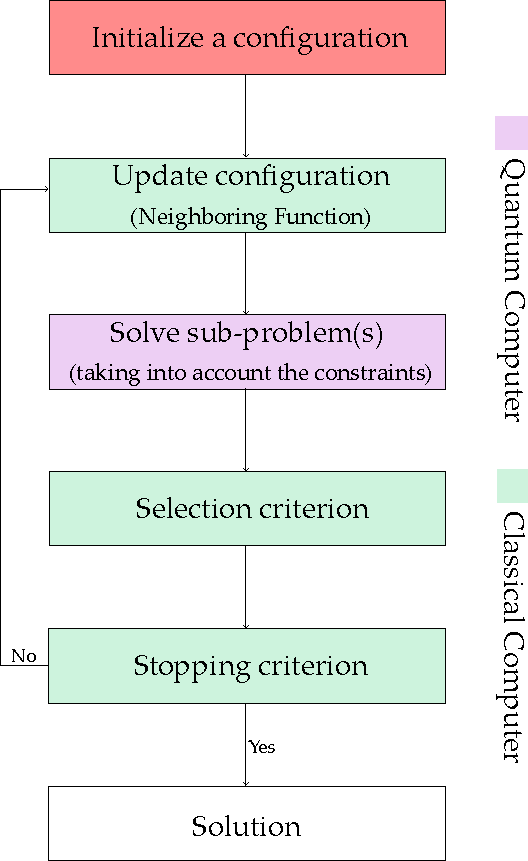
\includegraphics[width=0.5\textwidth]{Figures/SAQAProtocol_Layer 1.pdf} 
\caption{SA-QA protocol scheme.}
\label{fig:SA_QAProtocol}
\end{figure}
\begin{enumerate}
    \item Set the cost to a high value and initialize a configuration for the problem, i.e., annealing schedule, initial and final temperature, and a selection criterion.
    \item Randomly generate a new configuration by changing the values of the binary variables according to a neighboring function that generate a new configuration in one of this ways:
    \begin{enumerate}
        \item Randomly pick a binary variable with value 1 and set it to 0.
        \item Randomly pick a binary variable with value 0 and set it to 1.
        \item Randomly pick two binary variables with different values and swap them.
    \end{enumerate}
    \item Given the new configuration, solve the operational cost problem taking into account the constraints with a quantum annealing algorithm.
    \item Apply the selection criterion to keep or to discard the current configuration.
    \item Repeat steps 2 to 4 until a iteration index is equal to the upper value, then decrease the temperature and reset the iteration index.
    \item Outputs the current cost function value and its solution $\vec{x}$ when a stopping criterion is satisfied.
\end{enumerate}
Notice that the algorithm solve the master problem with a simulating annealing algorithm in a classical solver and then the sub-problem(s) -- which carries the constraints -- with the quantum computer, more precisely with a quantum annealer. For this reason, the sub-problem(s) must have binary constraints or integer if we do not want to deal with discretization errors. Hence, the approach as stated before is not for problems whose sub-problem(s) has real constraints meanwhile the master problem is more suitable for a quantum annealer.\\\\
In order to apply both simulated and quantum annealing to problems with real constraints, we have to reconsider or adapt the previous scheme.

%%%%%%%%%%%%%%%%%%%%%%%%%%%%%%%%%%%%%%%%%%%%%%%%%%%%%%%%%%%%%%%%%%%%%%%%%%%%%%%
% BD
%%%%%%%%%%%%%%%%%%%%%%%%%%%%%%%%%%%%%%%%%%%%%%%%%%%%%%%%%%%%%%%%%%%%%%%%%%%%%%%
\section{Benders' Decomposition}
The main idea behind Benders decomposition is that some problems simplify drastically if some variables are fixed, i.e., if some variables act as parameters. For this reason, the original problem is decompose into two problems with fixed variables. Firstly, a master problem with a subset $x^{m)}_{i} \subset \mathcal{W}$ of the original variables and its constraints is solved, then a sub-problem, which is the original problem with $x^{m)}_{i}$ fixed by the solution of the master problem, is solved. The solution of the master problem generates a lower bound, meanwhile the solution of the sub-problem generate an upper bound. Both problems are solved interactively according to some criteria until lower and upper bound are as close as the precision we want $\epsilon$.

%%%%%%%%%%%%%%%%%%%%%%%%%%%%%%%%%%%%%%%%%%%%%%%%%%%%%%%%%%%%%%%%%%%%%%%%%%%%%%%
% BD
%%%%%%%%%%%%%%%%%%%%%%%%%%%%%%%%%%%%%%%%%%%%%%%%%%%%%%%%%%%%%%%%%%%%%%%%%%%%%%%
\subsection{Classical Benders decomposition}
\textit{Classical Benders decomposition} (CBD) is a method to solve \textit{mixed integer programming} problems (MIP), but also MILP problems. These type of problems are combinatorial optimization problems, i.e., their goal is to find the combination of variables $x_{i}$ that minimises a given function, known as cost function subject to some integer constraints.\\\\
Suppose we are given a large optimization problem with many decision variables $\left(x_{0}^{m)}, x_{1}^{m)}, \hdots , x_{n}^{m)}, x_{0}^{s)}, x_{1}^{s)}\hdots x_{m}^{s)}\right)$ where the index $m$ indicates the variables associated with the master problem, and $s$ the variables associated with the sub-problem. The solution both problems find has to be consistent with the original problem, i.e., the constraints have to be fulfilled.\\\\
In the first iteration we have to fix the variables $x_{i}^{m)}$ to a feasible value and solve the sub-problem according to that fixed values. Once the sub-problem is solved
%%%%%%%%%%%%%%%%%%%%%%%%%%%%%%%%%%%%%%%%%%%%%%%%%%%%%%%%%%%%%%%%%%%%%%%%%%%%%%%
% BD: Multi-Cuts
%%%%%%%%%%%%%%%%%%%%%%%%%%%%%%%%%%%%%%%%%%%%%%%%%%%%%%%%%%%%%%%%%%%%%%%%%%%%%%%
\subsection{Hybrid Quantum-Classical Multi-cut Benders Approach}
In this section we present the protocol of a hybrid quantum-classical approach that has been applied to power system applications, see Ref.\,\cite{Paterakis2021HybridApplication}.\\\\


%----------------------------------------------------------------------------------------

% Define some commands to keep the formatting separated from the content 
\newcommand{\keyword}[1]{\textbf{#1}}
\newcommand{\tabhead}[1]{\textbf{#1}}
\newcommand{\code}[1]{\texttt{#1}}
\newcommand{\file}[1]{\texttt{\bfseries#1}}
\newcommand{\option}[1]{\texttt{\itshape#1}}

%----------------------------------------------------------------------------------------



